\section{Fundamentals and Related Work} \label{fundamentals_related_work}

Q-Learning is a known off-policy and model-free approach to train an agent based on temporal difference in an environment that can be modeled as a Markov Decision Process (MDP). An agent therefore does not necessarily use the policy it is trained for and does not know the transition probabilities and rewards in the MDP beforehand. \autoref{QLearning} shows the iterative update formula for the Q-values that an online model uses to choose the right action \cite{Geron2018}.

\begin{equation} \label{QLearning}
	Q_{k+1}(s,a) = (1-\alpha) Q_k(s,a) + \alpha(r + \gamma \max_{a'} Q_k(s',a')) 
\end{equation}

The problem with conventional Q-Learning is that in most of the cases the state dimension is far too high to explore and model the MDP entirely in foreseeable future. To deal with this problem the Q-values need to be approximated using a regression model. Deep neural networks have proven to be highly applicable for this task, which leads to the term of \textit{Deep-Q-Learning} and respectively \textit{Deep-Q-Networks} (DQN) for such network architectures. DQNs use the vectorized numerical state as its input and outputs the predicted Q-values. It learns through backpropagating the temporal difference error over each step for a single neuron. Note that for the Q-Learning algorithm a backpropagation is done after every step of the simulation. To avoid correlation between succeeding experiences an experience buffer is used to randomly sample a training batch in each step. In the following papers regarding DQN architectures shall be introduced as well as papers dealing with the bomberman environment for reinforcement learning. 

Paper \cite{vanHasselt2015} tackles the problem that the $max$ operator in \ref{QLearning} often leads to overoptimistic value estimates as the DQN uses the same Q-values to both select and evaluate an action. It therefore changes the iterative update formula to \ref{DoubleQLearning}.

\begin{equation} \label{DoubleQLearning}
	Q_{k+1}(s,a) = (1-\alpha) Q_k(s,a) + \alpha(r + \gamma Q'_k(s', arg\max_{a'} Q_k(s',a'))) 
\end{equation}

Now a target DQN is used to separate the determination of the greedy policy, which is still done by the online network, from the Q-value estimation. Using this double DQN approach results in less overestimated Q-values and therefore better policies by more accurate Q-value estimates. It also makes the learning process more stable and reliable. The weights are copied from the online network to the target network after a fixed amount of episodes.

Another optimization was introduced in paper \cite{Wang2016}. It changes the architecture of the DQN by splitting it into two separate value streams. One stream estimates the state value function and the other one the state-dependent action advantage function. Both streams are then combined again using a special aggregating layer to produce an estimate of the Q-values (see \autoref{fig:duelingDQN}).  

\begin{figure}[ht]
	\centering
	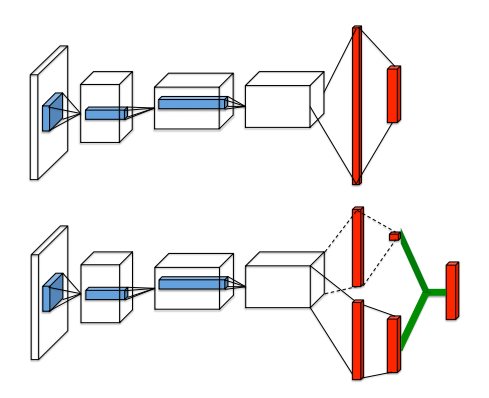
\includegraphics[width=0.6\linewidth]{figures/duelingDQN.png}
	\caption{Architecture of a normal DQN (top) compared to a dueling DQN (bottom)}
	\label{fig:duelingDQN}
\end{figure}

The state-dependent action advantage function is defined as

\begin{equation} \label{advfunction}
	A^{\pi}(s,a) = A^{\pi}(s,a) - V^{\pi}(s)
\end{equation}

and measures the importance of each action. The special aggregating layer uses \autoref{aggregation} to estimate the Q-values while also tackling the issue of identifiability. 

\begin{equation} \label{aggregation}
	Q(s, a; \theta, \alpha, \beta) = V(s; \theta, \beta) + (A(s, a; \theta, \alpha) - \frac{1}{\abs{A}} \sum_{a'}A(s, a'; \theta, \alpha)) 
\end{equation}

Using the dueling architecture approach an agent can learn which states are valuable independently of each action, which is esspecially useful in case actions do not influence the environment in any useful way. This leads to a better policy evaluation in the presence of many similar-valued actions. Also when looking at the last layer of a conventional DQN (see \autoref{fig:duelingDQN}) it usually becomes much more sparse and biased. As the state value is modeled as a single neuron in the dueling architecture, learning the state value function becomes much more efficient.

% TODO: Prioritized replay buffer

There are several other improvements mentioned in the rainbow paper \cite{Hessel2017} like multi-step learning, distributional reinforcement learning and noisy nets, but these are out of the scope for this small research project. 